\documentclass{beamer}
\usetheme{Frankfurt}
\usepackage{tikz}
\usepackage{minted}
\usefonttheme{professionalfonts}
\usecolortheme{sidebartab}
\usepackage{xcolor}
\usepackage{hyperref}

\usetikzlibrary{chains, shadows.blur, trees}
%Information to be included in the title page:
\title[\url{https://google.com}] %optional
{LLVM \& HPSSA}

\subtitle{Hot Path SSA Form in LLVM}

\author[VIP1 \& VIP2] % (optional, for multiple authors)
{Presented By Abhay\inst{1} \& Muzzammil\inst{1}}

\institute[IDK] % (optional)
{
	\inst{1}%
	IIT Kanpur\\
	PRAISE Group
}

\date[01/03/2022] % (optional)
{Dr. Subhajit Roy, Dr. Awanish Pandey, Mr. Sumit Lahiri}

\begin{document}
\frame{\titlepage}
\footnotesize
\section{LLVM Modifications}

\begin{frame}[fragile]
	\frametitle{What we modified in LLVM Source?}
	\begin{itemize}
		\item New \mintinline[]{css}{llvm::intrinsic} signature, \mintinline[]{css}{"llvm.tau"} to support addition and removal of $\tau$-functions to the LLVM SSA IR representation. 
	\end{itemize}
	\begin{minted}{python}
	+ //===---------- intrinsic for tau ---------------=====//
	+ def int_tau : DefaultAttrsIntrinsic<[llvm_any_ty],
	+                               [llvm_vararg_ty],
	+                               []>;
	\end{minted}
\end{frame}
\footnotesize
\begin{frame}[fragile]
\frametitle{What we modified in LLVM Source?}
\begin{itemize}
	\item Modified \mintinline[]{css}{Verifier::verifyDominatesUse()} function since we don't want our intrinsic to interfere with \mintinline[]{css}{dominators} computation.  
\end{itemize}
\begin{minted}{python}
+ //===---------- Changes for tau.intrinsic ---------------=====//
void Verifier::verifyDominatesUse(Instruction &I, unsigned i) {
  Instruction *Op = cast<Instruction>(I.getOperand(i));
  +  if (CallInst *CI = dyn_cast<CallInst>(&I)) {
  +    Function *CallFunction = CI->getCalledFunction();
  +    if (CallFunction != NULL && CallFunction->getIntrinsicID() ==
  +        Function::lookupIntrinsicID("llvm.tau")) {
  +      return;
  +    }
  +  }
	\end{minted}
\end{frame}

\section{LLVM : HPSSA Pass}
\footnotesize
\begin{frame}
	\frametitle{\texttt{HPSSAPass} : Overview}
	\begin{itemize}
		\item Implemented \mintinline[]{css}{llvm::HPSSAPass} pass using the new LLVM Pass Manager. 
		\item Pass \mintinline[fontsize=\footnotesize]{css}{HPSSAPass::run(Function \&F, ...)}  runs over a \mintinline[]{css}{llvm::Function} and inserts \mintinline[]{css}{"llvm.tau"} intrinsic calls with speculative and safe arguments at strategic positions in the LLVM IR as described in the previous slides.
	\end{itemize}
	Key HPSSA Data Structures :  
	\begin{itemize}
		\item Hot Path Set using \mintinline[]{css}{llvm::BitVector}.
		\item Definition Accumalator, \texttt{defAccumalate} as a map  \mintinline[]{python}{std::map<{PHINode*,BasicBlock*}, {Value*,BitVector}>}.
		\item Variable Renaming Stack as a map, \mintinline[]{python}{std::map<Value*,Value*>}
	\end{itemize}
\end{frame}

\begin{frame}{HPSSA Transformation}
	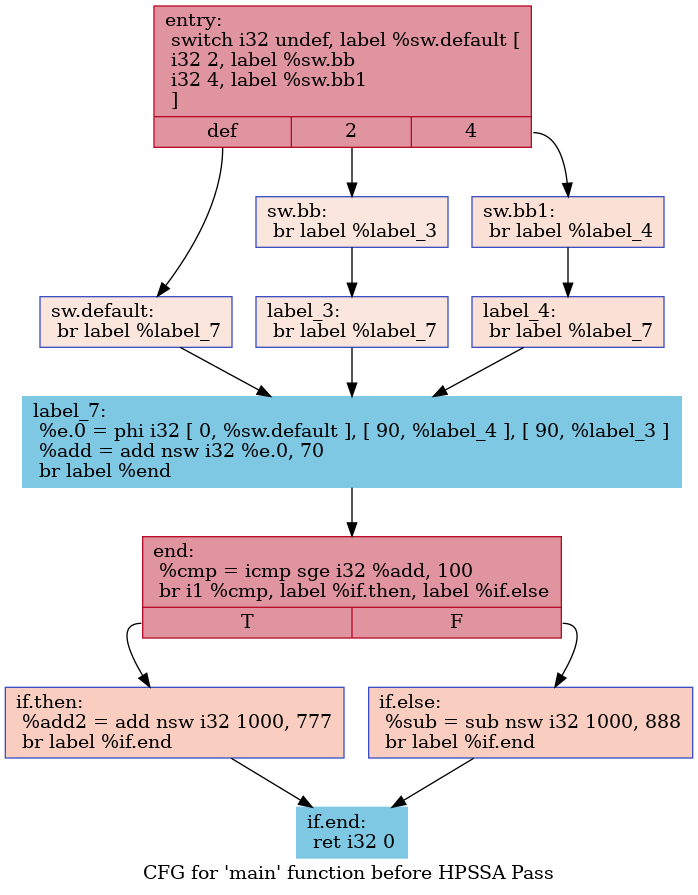
\includegraphics[width=5.3cm,height=7.5cm]{baseline.dot.png}
	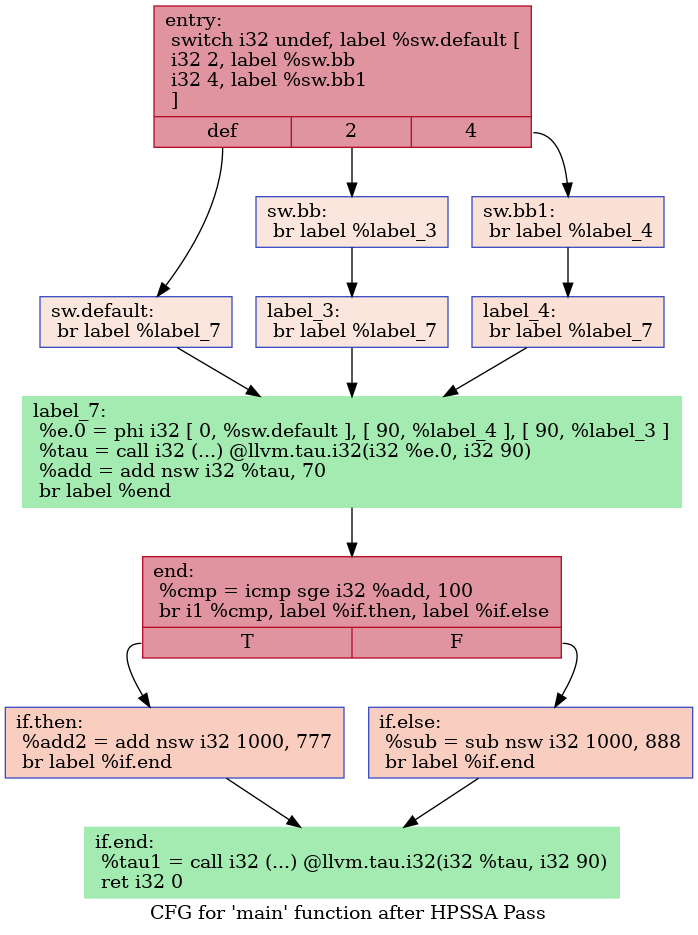
\includegraphics[width=5.3cm,height=7.5cm]{afterHPSSA.dot.png}
\end{frame}

\begin{frame}
	\frametitle{\texttt{HPSSAPass} : Main \& Destruction Pass}
	\begin{itemize}
		\item \mintinline[fontsize=\footnotesize]{css}{HPSSAPass::run(Function \&F, FunctionAnalysisManager \&AM)} 
		\item \mintinline[fontsize=\footnotesize]{css}{llvm::Function::RPOT()}.
		\item \mintinline[fontsize=\footnotesize]{css}{llvm::successors()}.
		\item \mintinline[fontsize=\footnotesize]{css}{llvm::DominatorTreeAnalysis} and \mintinline[fontsize=\footnotesize]{css}{llvm::dominates()}.
		\item Replace use of \mintinline[]{css}{phi's} with \mintinline[]{css}{tau} variables using \texttt{renaming} stack.
		\item Out of HPSSA Form. 
	\end{itemize}
\end{frame}

\begin{frame}
	\frametitle{\texttt{HPSSAPass} : Auxilliary Functions}
	\begin{itemize}
		\item \mintinline[fontsize=\footnotesize]{css}{HPSSAPass::getProfileInfo(Function \&F)}
		\item \mintinline[fontsize=\footnotesize]{css}{HPSSAPass::getCaloricConnector(Function \&F)}
		\item \mintinline[fontsize=\footnotesize]{css}{HPSSAPass::Search(BasicBlock \&BB, DomTreeNode \&DTN})
	\end{itemize}
\end{frame}

\section{SSCCP Pass in LLVM}

\begin{frame}
	\frametitle{New Additions to SCCP Pass}
	\begin{itemize}
		\item Modified the existing SCCP Pass to add in \mintinline[fontsize=\footnotesize]{css}{SCCPInstVisitor::visitTauNode()} function similar to \mintinline[fontsize=\footnotesize]{css}{SCCPInstVisitor::visitPHINode()}, which handles the special \mintinline[fontsize=\footnotesize]{css}{"llvm.tau"} intrinsic instructions added for $\tau$-functions.
		\item Added a new lattice element type \mintinline[fontsize=\footnotesize]{css}{"spec_constant"} in \mintinline[fontsize=\footnotesize]{css}{ValueLattice} class supporting operations on speculative constants. 
		\item Added new functions in the \mintinline[fontsize=\footnotesize]{css}{SCCPInstVisitor} and \mintinline[fontsize=\footnotesize]{css}{SCCPSolver} class to handle operations on speculative constants using \mintinline[fontsize=\footnotesize]{css}{markSpeculativeConstant()} function.
	\end{itemize}
\end{frame}

\begin{frame}[fragile]
	\frametitle{Further Modifications}
	\begin{itemize}
		\item Modified the \mintinline[fontsize=\footnotesize]{css}{SCCPInstVisitor::mergeIn()} function to handle lattice ''meet" operation for the new speculative constants introduced.  
		\item Since we added the $\tau$-functions as an \mintinline[fontsize=\footnotesize]{css}{"llvm.tau"} intrinsic which is essentially an \mintinline[fontsize=\footnotesize]{css}{llvm:CallInst} type, we modified all appropriate visit and marking functions in \mintinline[fontsize=\footnotesize]{css}{SCCPInstVisitor, SCCPSolver} and \mintinline[fontsize=\footnotesize]{css}{SCCPPass} to handle this case separately by calling \mintinline[fontsize=\footnotesize]{css}{visitTauNode()}.
		\item Modified utility functions in \mintinline[fontsize=\footnotesize]{css}{SCCPInstVisitor} and \mintinline[fontsize=\footnotesize]{css}{SCCPSolver} class to print marking of speculative constants and related operations for debugging purpose.
	\end{itemize}
\begin{minted}[fontsize=\footnotesize]{css}
...
[BBWorkList] Visiting LLVM Instrinsic : llvm.tau (call)
Visiting Tau Instruction
Speculative Operand : , speculative constant
Speculative Operand : llvm.tau.i32, speculative constant
Merged speculative constant into   %tau = call i32 (...) 
	@llvm.tau.i32(i32 %e.0, i32 90) : speculative constant
ValueLattice (TauState) : speculative constant
\end{minted}
\end{frame}

\begin{frame}[fragile]
\begin{minted}[fontsize=\footnotesize]{cpp}
int main() {
	int a = 1000, z, c, e = 0;
	switch(c) {   
		case 2 : goto label_3; break;
		case 4 : goto label_4; break;
		default : goto label_7;
	}
	label_3:
		e = 90;
		goto label_7;
	label_4:
		e = 100 - 10;
		goto label_7;
	label_7:
		e = e + 70;  // e in rhs is 90.
		goto end;
	end:
		if (e >= 100) {  // e is greater than 100 always
			a = a + 777;
		} else {
			a = a - 888;
		}
	return 0;
}
\end{minted}
\end{frame}

\begin{frame}
	\frametitle{SSCCP with an Example}
	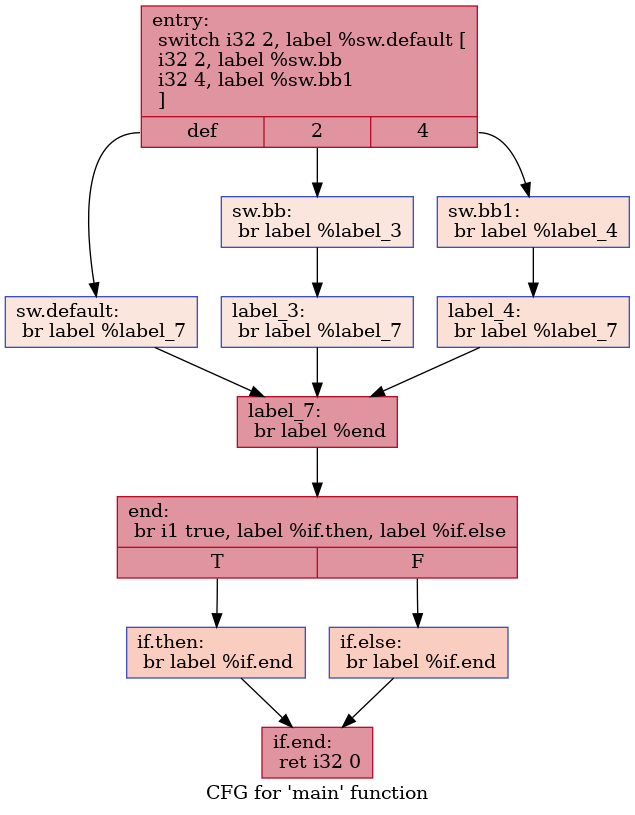
\includegraphics[width=5.3cm,height=7.5cm]{SCCP_BASELINE.dot.png}
	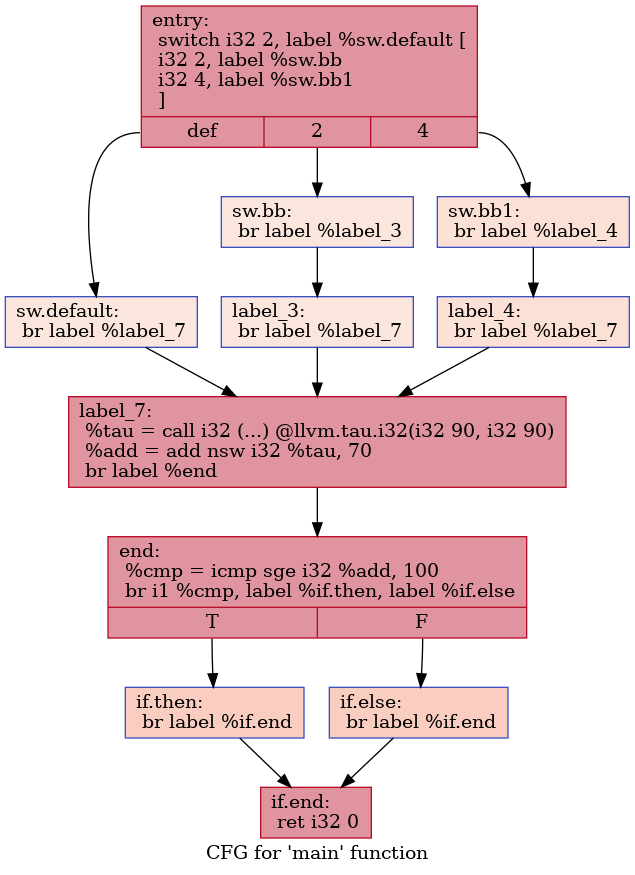
\includegraphics[width=5.3cm,height=7.5cm]{specSCCP_HPSSA.dot.png}
\end{frame}

\end{document}